\documentclass[9pt,twocolumn,twoside]{../../styles/osajnl}
\usepackage{fancyvrb}
\journal{i524} 

\title{Jupyter Notebook vs Apache Zeppelin - A comparative study}

\author[1,*]{Sriram Sitharaman}

\affil[1]{School of Informatics and Computing, Bloomington, IN 47408, U.S.A.}

\affil[*]{Corresponding authors: srirsith@iu.edu}

\dates{\today}

\ociscodes{Jupyter, Zeppelin, Notebook, Comparison}

% replace this with your url in github/gitlab
\doi{\url{https://github.com/cloudmesh/classes/blob/master/docs/source/format/report/report.pdf}}


\begin{abstract}


With the development of new technologies for the purpose of exploring, analysing and visualizing big datasets, there exists a growing demand of a collaborative platform that combines the process of data analysis and visualization.The idea of computer notebooks has been around for a long time, starting with the introduction of Matlab and Mathematica. Two such platforms: Apache Zeppelin and Jupyter notebook are taken in to consideration for comparison. Both of them were ranked against characteristics such as their ability to support multiple programing techniques, multi-user support and integrated visualization.\newline
\end{abstract}

\setboolean{displaycopyright}{true}

\begin{document}

\maketitle
\tableofcontents % Print the contents section
\section{Introduction - Jupyter Notebook}
Jupyter notebook, part of project Jupyter is the third version of IPython notebook. It is a web based interactive development environment and supports multiple programming languages (Python, Julia, R etc.) \cite{www-jupyter-wiki}. It started supporting Julia, Python and R in its initial release, hence the term Jupyter. The web based interative environment provided by Jupyter is facilitated through a notebook interface which contains the programming code written by the user as well mark down elements and outputs that are generated as result of the written code\cite{www-jupyter-notebook}. Hence, Jupyter Notebook documents allows a seemless view of the code written and the corresponding output (graphs,tables,etc.). The Jupyter Notebook app is a client-server application as shown in the figure \ref{fig:arch} that can be run on a local machine for personal use and can be accessed without the internet, or can be installed in a remote server which can be accessed via an internet connection. The final component of the Jupyter Notebook is the kernel which performs the execution of code written by user. Jupyter comes with a native Ipython kernel (supporting Python), and also supports 80+ programming languages' kernels \cite{www-jupyter-kernel}.
\begin{figure}[h]
\begin{center}
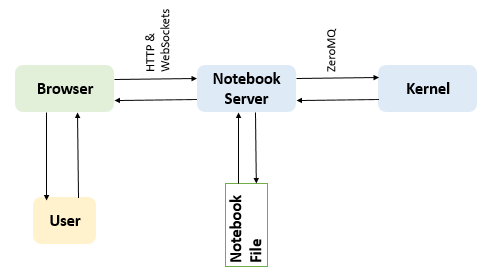
\includegraphics[width =\linewidth,height=2.5in]{images/JupyterNotebook}
\caption{Jupyter Architecture \cite{www-jupyter-arch}}
\label{fig:arch}
\end{center}
\end{figure}
\section{Introduction - Apache Zeppelin}

Apache Zeppelin \cite{www-zeppelin}, similar to Jupyter notebook, is also a web based interactive notebook but aimed towards supporting big data and data analytics. It supports multiple programming languages. It is useful in exploration of data, creation of visualizations and sharing insights, as web pages, with various stakeholders involved in a project. It supports a range of programming languages like Scala, Spark SQL, Shell, etc with the default being scala. Zeppelin has an architecture similar to Jupyter notebook with an exception that notebook in Zeppelin supports the integration of multiple programming languages in a single notebook. Zeppelin's notebook is shipped with some basic charts which can be used to visualize output generated by any supported programming language. Apart from that, it has the option of pivot charts and Dynamic forms that can be generated inside the notebook interface. 

\section{Comparison}

This section would compare the following aspects of Apache Zeppelin and Jupyter notebook:
\begin{enumerate}
    \item Interpreter configuration
    \item Interface
    \item Supported Languages
    \item Visualization
    \item Multi-user capability
    \item Community Support
\end{enumerate}

\subsection{Interpreter configuration}

Zeppelin interpreter is a language/data-processing-backend that can be plugged into Zeppelin notebook. Currently, Zeppelin supports over 30 interpreters such as Scala ( with Apache Spark ), Python ( with Apache Spark ), Spark SQL, JDBC, Markdown, Shell, etc \cite{www-zeppelin-int}. Zeppelin has a separate Interpreter configuration page that you can be accessed for multiple language parameters. For instance, Spark home directory as well as spark master string can be modified to our preference. It would create the Spark Context automatically so you don't need to deal with it in each notebook.For example, to use Scala code in Zeppelin, "\%spark" has to be included to load the interpreter. Apache Zeppelin provides several interpreters as community managed interpreters \cite{www-zeppelin-int-install} which can be installed at once if \textbf{netinst} binary package has been installed. It also supports installation of 3rd party interpreters.\\

For Jupyter, IPython is the default kernel defined as Kernel zero, which can be obtained through the kernel \textbf{ipykernel}. Jupyter supports the use of 80+ kernels and \cite{www-jupyter-kernel} shows how each of them can be installed, required dependencies and the correponding programming language version needed.

\subsection{Interface}
Zeppelin leverages a common UI framework with Bootstrap and Angular.js for the notebook interface. It is a easy to use interface with the support for creating dynamic forms within Zeppelin's notebook for which input can be obtained from a programming languages' output. Zeppelin provides an interface that is similar to RShiny's interactive web interface which allows user to manipulate in the front end rendered using Javascript with R running in the background \cite{www-rshiny}. 

Jupyter, on the other hand has a simple interface that is not user interactive as Zeppelin. When jupyter notebook is launched, the first page that is encountered is the Notebook Dashboard which shows the notebook files that has been created already and residing in the server. A new notebook can be created that is associated to a specific programming language's kernel (Python 2/Python 3/ R etc.) \cite{www-jupyter-ui}. It's interface simple interface having a cell where the code can be written. Once the code is executed, the area below the cell would display the corresponding output.
\begin{figure*}[hbt]
\begin{center}
\centering
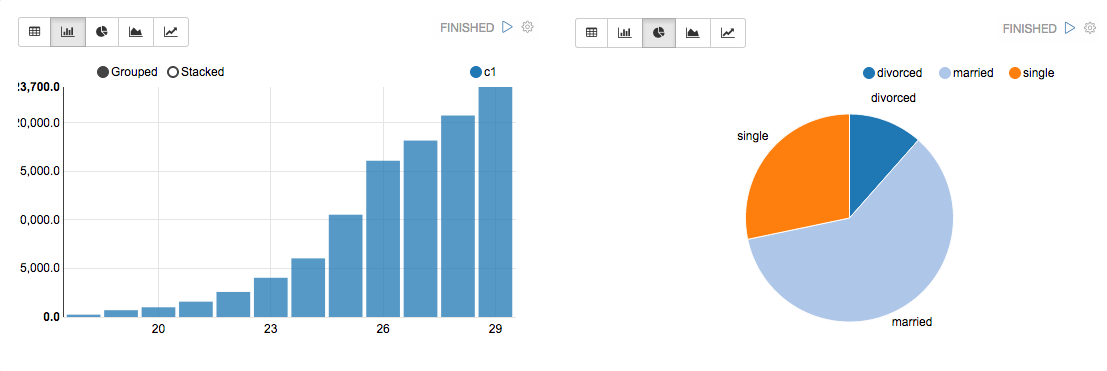
\includegraphics[width =\linewidth,height=2.5in]{images/graph}
\caption{Snapshot of Integrated graph - Apache Zeppelin \cite{www-zeppelin}}
\label{fig:graphZep}
\end{center}
\end{figure*}
\subsection{Supported Languages}
Zeppelin has the support for the 16 interpreters mentioned in Table \ref{langsupport}. Since Apache Zeppelin has the default interpreter as spark which is a one of the major technology used for solving big data problems, the list includes interpreters like hbase, cassandra, elastic search etc. that works along with spark in solving big data problems.To overcome the limitation of these list of interpreters, Zeppelin provides the support for writing our own interpreter as described in \cite{www-zeppelin-int-own}. 

\begin{table}[hbt]
\caption{Programming languages supported by Apache Zeppelin}
\begin{tabular}{|l|1|1|1|}
\hline
alluxio       & file   & jdbc  & md         \\
angular       & flink  & kylin & postgresql \\
cassandra     & hbase  & lens  & python     \\
elasticsearch & ignite & livy  & shell      \\ \hline
\end{tabular}
\label{langsupport}
\end{table}

Jupyter, on the other hand has a huge list of about 80+ kernels being supported currently \cite{www-jupyter-kernel}. Though Jupyter has an upperhand over Zeppelin over the number of supported programming languages, it lags behind Zeppelin in the support of using different programming language in the same notebook. 

\subsection{Visualization}
Zeppelin provides the freedom to play around with various types of chart as shown in figure \ref{fig:graphZep}. It provides charting options by default for the output generated as a result of execution of code. The Apache Zeppelin community has been working on Project Helium \cite{www-helium-wiki}, which aims to seed growth in all kinds of visualizations. This follows the model created by pluggable interpreters. Helium aims to make adding a new visualization simple, intuitive and can be accessed through a packaged code.

Jupyter, on the other hand has no charting options by default. Hence, it relies on existing charting libraries from the programming language that the notebook uses.

\subsection{Multi-user capability}
Zeppelin is still working towards providing multi user capability. Jupyter Hub \cite{www-jupyterhub} provides multiple user support for Jupyter. It simple to setup because it leverages the Linux users and groups to provide authentication.Three subsystems make up JupyterHub as shown in Figure \ref{fig:jhub}.
Each user cannot touch or see any other users because it's restricted at the OS layer. However, Jupyter Hub has to be maintained in a single server which would provide access to multiple users.
\begin{enumerate}
     \item a multi-user Hub (tornado process)
     \item a configurable http proxy (node-http-proxy)
     \item multiple single-user Jupyter notebook servers (Python/IPython/tornado) 
\end{enumerate}
\begin{figure}[h]
\begin{center}
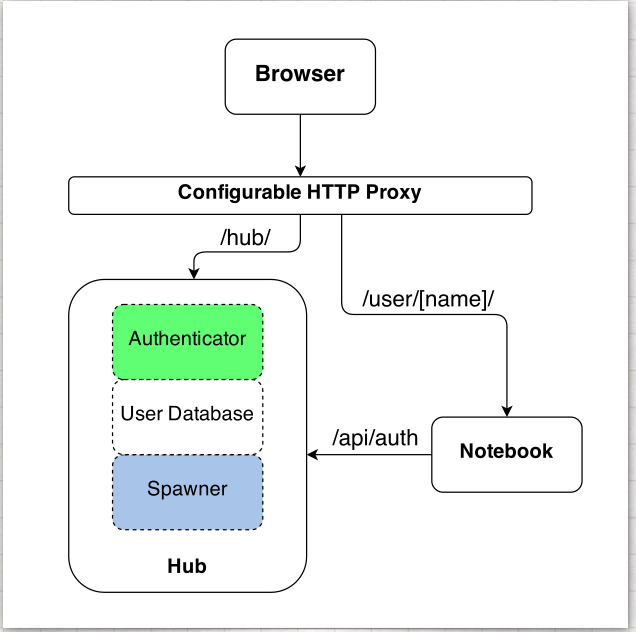
\includegraphics[width =3in,height=2.5in]{images/jhub}
\caption{Jupyter HUB Architecture \cite{www-jupyterhub}}
\label{fig:jhub}
\end{center}
\end{figure}

\subsection{Community support}

Zeppelin is still in the incubation stage of Apache. It is progressing very slowly relatively to the status of Jupiter today. However, since Jupyter has a long history as IPython, there is lot of support for Jupyter in the online communtiy. A simple google search for the term \textbf{IPython} gives around ~1.3 million results whereas for \textbf{Apache Zeppelin}, it is around ~0.45 million. Apache Zeppelin is working with NFLabs, Twitter, Hortonworks, MapR, Pivotal, and IBM among many others delivering new features and fix issues in its platform \cite{www-horton-zeppelin}.

\section{Alternatives to Jupyter and Apache Zeppelin}
\subsection{Beaker Notebook}
The Beaker Notebook is built on top of IPython kernel and  was designed from the start to be a fully polyglot notebook \cite{www-beaker}. It currently supports Python, Python3, R, Julia, JavaScript, SQL, Java, Clojure, HTML5, Node.js, C++, LaTeX, Ruby, Scala, Groovy, Kdb. It follows a cell type interface similar to Jupyter and Zeppelin and allows the user to use multiple programming languages across different cells in the same notebook. (i.e.) For example, the output of the code written in R in cell 1 can be accessed by a block of code written in Python in cell 2 for further manipulations.

\subsection{SageMath}
Sagemath is a is a free open-source mathematics software system \cite{www-sagemath} built for creating an open source alternative to Magma, Maple, Mathematica, and MATLAB. It is build on top of  existing open-source packages: NumPy, SciPy, matplotlib, Sympy, Maxima, GAP, FLINT, R etc. It also offers a notebook type interface and the Sage Notebook recently moved to the cloud with SageMathCloud in collaboration with Google’s cloud services.

\section{Conclusion}

The very need for experiments, explorations, and collaborations in scientific programming community is addressed by the evolution of these notebooks.Considering these into account, Apache Zeppelin is gaining upper hand over Jupyter in providing a fluid environment to solve big data problems apart from it being in the initial stages of defining multi-user support and relatively small community. With Zeppelin being a part of Apache community, it would be understandable that there would be constant growth and updates. This can be strengthened from the fact that Apache Zeppelin is in the initial stages of developing Helium which would make visualization easy to use for big data problems.

\bibliography{references}

\end{document}
